\begin{Example}[ashford]{Breathlessness and wheeze in coal miners}
In \exref{ex:wheeze1} we examined the association between the occurrence
of two pulmonary conditions, breathlessness and wheeze,
among coal miners, classified by age \citep{AshfordSnowden:70}.
\figref{fig:pie2x2wh1} showed fourfold displays focused on the odds ratio
for the co-occurrence of these symptoms,
and \figref{fig:pie2x2wh2} plotted these odds ratios against age directly.
Here, we consider models which examine the changes in prevalence of
the two symptoms over age, together with the changes in their association.

As a first step, we calculate the log odds for breathlessness and for
wheeze, and the log odds ratio for their association
in each $2 \times 2$ table. These values are shown in \outref{out:ashford.1}.
The log odds ratios are the same values plotted in \figref{fig:pie2x2wh2}
(but the youngest age group was not included in the earlier analysis).
\begin{listing}
data ashford;
   input age @;
   age2 = age**2;
   do breath = 1, 0;
      do wheeze = 1, 0;
         input count @;
         output;
         end;
      end;
   label breath='Breathlessness'
      wheeze='Wheeze'
      age='Age Group';
datalines;
20     9    7      95 1841
25    23    9     105 1654
30    54   19     177 1863
35   121   48     257 2357
40   169   54     273 1778
45   269   88     324 1712
50   404  117     245 1324
55   406  152     225  967
60   372  106     132  526
;
proc transpose out=ashford1 prefix=r;
   var count;
   by age;

data ashford1;
   set ashford1;
   drop _name_;
   logit1 = log( (r1 + r2 + .5) / (r3 + r4 + .5) );
   logit2 = log( (r1 + r3 + .5) / (r2 + r4 + .5) );
   logodds= log( ((r1+.5)*(r4+.5))/((r2+.5)*(r3+.5)) );
   label logit1='Logit(Breathlessness)'
      logit2='Logit(Wheeze)';
proc print;  id age;
\end{listing}

\begin{Output}[htb]
\caption{Empirical logits and log odds ratios for breathlessness and wheeze}\label{out:ashford.1}
\small
\verbatiminput{ch7/out/ashford.1}
\end{Output}

Plotting both logits and the log odds against age gives the graph shown
in \figref{fig:ashford1}.
The plotting step is straight-forward and is not shown.
We see that both symptoms, while quite rare among young miners, increase
steadily with age (or years working in the mine).
There is a hint of curvilinearity, particularly in the logit for
breathlessness.
The decline in the odds ratio with age reflects selection, as miners
who had retired for health or other reasons were excluded from the
study.
%% one figure
\begin{figure}[htb]
  \centering
  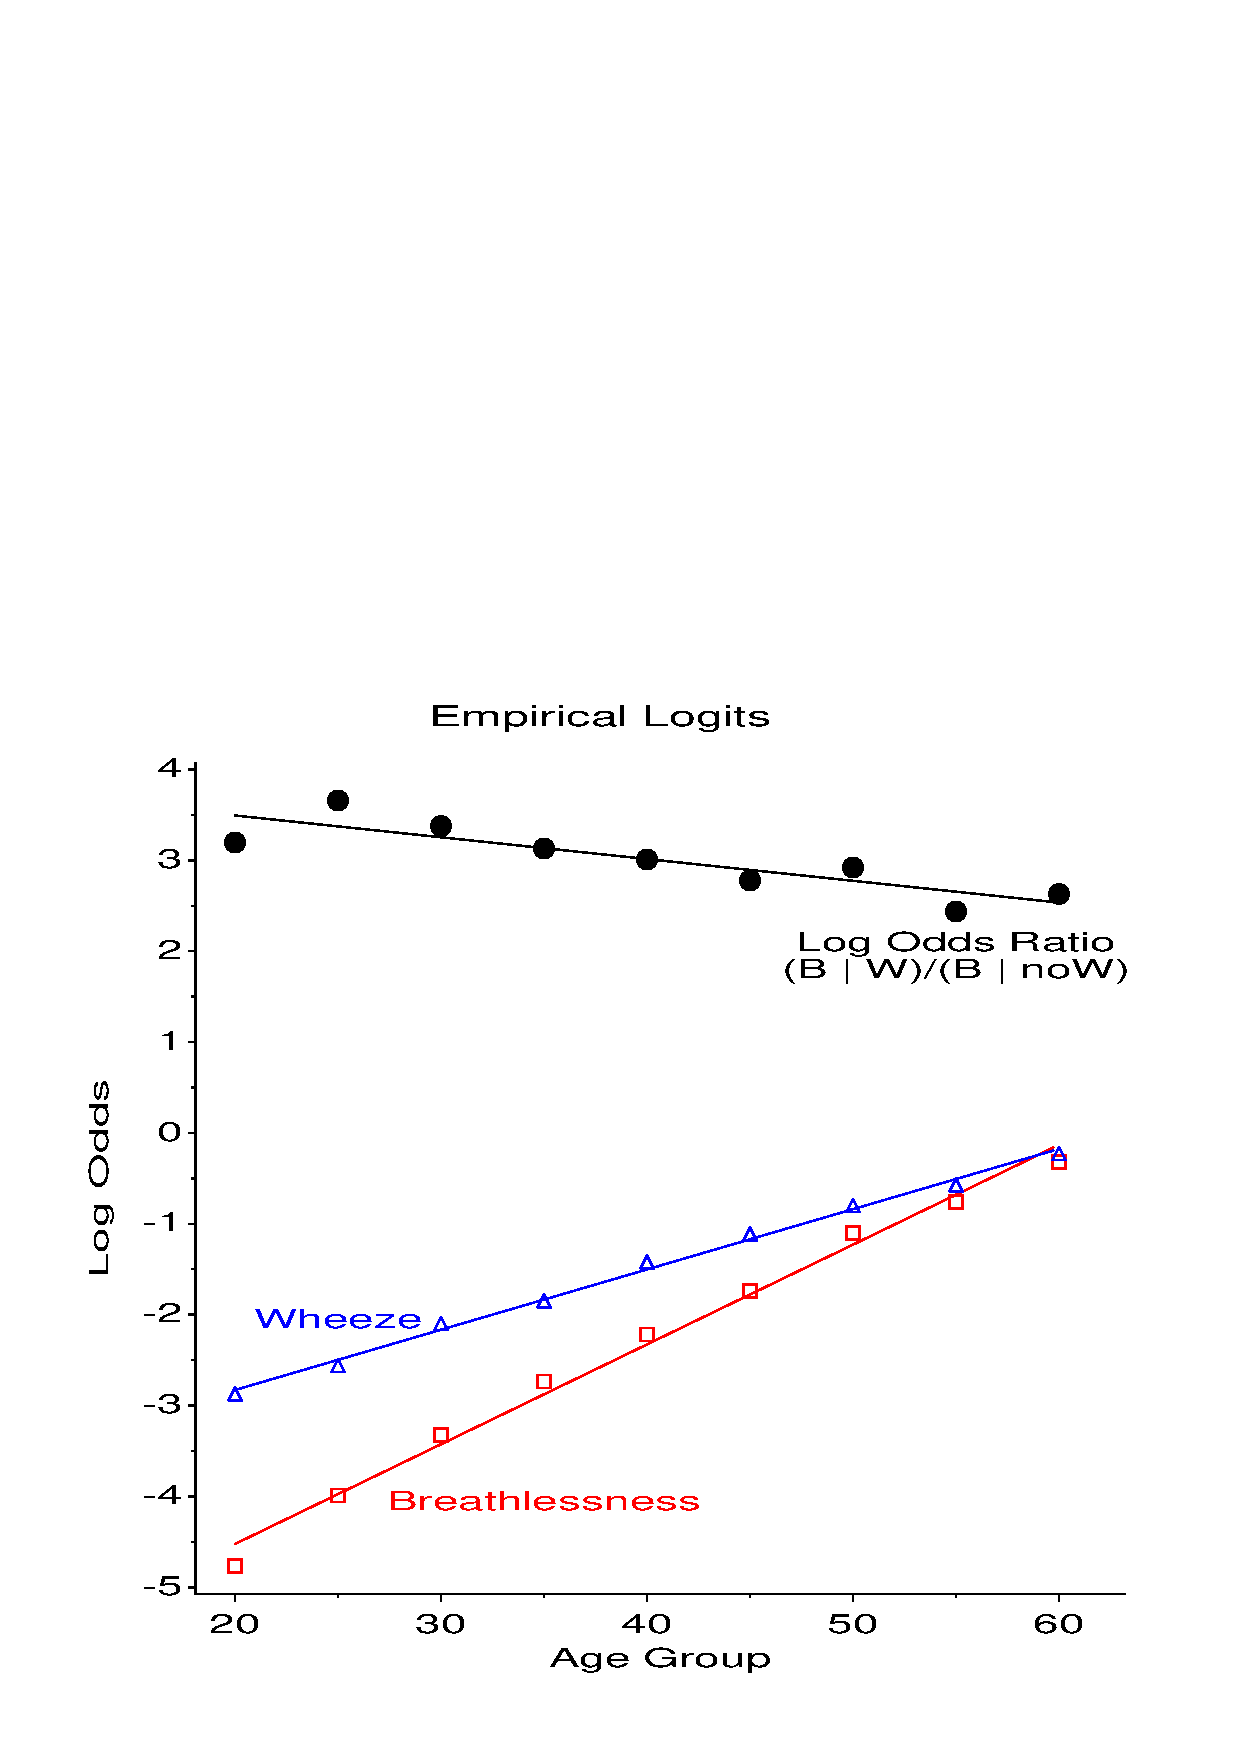
\includegraphics[scale=.6]{ashford1}
  \caption[Empirical logits and log odds ratios for breathlessness and wheeze]{Empirical logits and log odds ratios for breathlessness and wheeze.
  The lines show separate linear regressions for each function.}%
  \label{fig:ashford1}
\end{figure}

We can fit ordinary \loglin\ models to these data as shown below,
giving \LR\ goodness-of-fit \GSQ\ values shown in \tabref{tab:ashmod}.
Note that in Models 0--2, age is treated as a 9-level factor.
In Models 3--4, age is treated as a quantitative variable
(symbolized as $x$ in the model terms), by declaring
\pname{age} and \pname{age2} ($x^2$) in a \stmt{DIRECT}{CATMOD}.%
\footnote{In these model formulae, a term like $[Bx^2]$
refers to a quadratic model, $\eta_1 = \alpha_1 + \beta_{11} x + \beta_{11} x^2$ in \eqref{eq:bilogit1}}
\PROC{CATMOD} does not allow quantitative variables to appear
on the left-hand side in a \stmt{MODEL}{CATMOD}.
Consequently, these models are fit in a separate \PROC{CATMOD}
step, where they are expressed as \verb|_RESPONSE_*AGE| and
\verb|_RESPONSE_*AGE2| on the right-hand side.
%% input: /users/faculty/friendly/sasuser/catdata/ash1.sas
%% last modified: 16-Nov-98 13:44
\begin{listing}
title 'Loglinear models for B and W';   
proc catmod order=data data=ashford;
   weight count;
   model breath*wheeze*age = _response_ / 
      ml noiter noresponse noprofile nodesign nogls;
   loglin breath wheeze age / title='0: Minimal model: [B] [W] [A]';
run;
   loglin breath|wheeze age / title='1: Null age: [BW] [A]';
run;
   loglin breath|wheeze breath|age wheeze|age/ title='2: [BW] [BA] [WA]';

proc catmod order=data data=ashford;
   weight count;
   direct age age2;
   model breath*wheeze = _response_ _response_*age/ 
      ml noiter noresponse noprofile nodesign nogls;
   loglin breath|wheeze / title='3: [BW] [Bx] [Wx]';
run;
   model breath*wheeze = _response_ _response_*age _response_*age2/ 
      ml noiter noresponse noprofile nodesign nogls;
   loglin breath|wheeze / title='4: [BW] [Bx^2] [Wx^2]';
run;

\end{listing}

%\begin{table}[htb]
% \caption{Loglinear models fit to Ashford \& Snowden data}\label{tab:ashmod}
% \begin{center}
% \begin{tabular}{cl rrrr}
%  \hline
%  Model & Terms            & df & \GSQ & $p$-value & \GSQ /df \\ 
%  \hline
%  0 & $[B]  [W]  [A]$      & 25 & 6939.07 & 0.0000 & 277.56 \\ 
%  1 & $[BW] [A]$           & 24 & 2701.94 & 0.0000 & 112.58 \\ 
%  2 & $[BW] [BA] [WA]$     &  8 & 26.69   & 0.0008 & 3.34 \\ 
%  3 & $[BW] [Bx] [Wx]$     & 21 & 41.46   & 0.0049 & 1.97 \\ 
%  4 & $[BW] [Bx^2] [Wx^2]$ & 18 & 17.60   & 0.4825 & 0.97 \\ 
%  \hline
% \end{tabular}
% \end{center}
%\end{table}
%

% latex table generated in R 3.0.1 by xtable 1.7-3 package
% Thu May 08 11:49:32 2014
\begin{table}[htb]
 \caption{Loglinear models \func{glm} fit to Ashford \& Sowden data}\label{tab:ashmod}
\centering
\begin{tabular}{rlrrrrr}
  \hline
  Model   & Terms & LR Chisq & \GSQ & Pr($>$Chisq) & AIC & BIC \\ 
  \hline
  cm.glm0 & $\LLM{B, W, A}$ & 6939.07 & 25 & 0.0000 & 6889.07 & 6693.73 \\ 
  cm.glm1 & $\LLM{BW, A}$ & 2701.94 & 24 & 0.0000 & 2653.94 & 2466.42 \\ 
  cm.glm2 & $\LLM{BW,BA,WA}$ & 26.69 & 8 & 0.0008 & 10.69 & -51.82 \\ 
  cm.glm3 & $\LLM{BWx,BA,WA}$ & 6.80 & 7 & 0.4498 & -7.20 & -61.89 \\ 
   \hline
\end{tabular}
\end{table}



Model 0 is the minimal model of mutual independence; Model 1 allows
association of breathlessness and wheeze, but independent of age.
Neither of these makes any sense, given what we have seen graphically.
Model 2 allows both breathlessness and wheeze to depend on age as a factor.
The quantitative models for age, Models 3 and 4
correspond to what is apparent in \figref{fig:ashford1}.
Model 3 is equivalent in goodness-of-fit
to the bivariate \loglin\ model \eqref{eq:eta3},
but is parameterized in terms of generalized logits
\begin{equation*}
\left(
\begin{array}{c}
l _{11,22} \\
l _{12,22} \\
l _{21,22}
\end{array}
\right) =
\left(
\begin{array}{c}
\log \pi_{11} / \pi_{22} \\
\log \pi_{12} / \pi_{22} \\
\log \pi_{21} / \pi_{22}
\end{array}
\right) =
\left(
\begin{array}{c}
\alpha _1+\beta _1 x \\
\alpha _2+\beta _2 x \\
\alpha _{12}+\beta _{12} x \\
\end{array}
\right)   %\label{eq:biloglin}
\period
\end{equation*}
Model 4 adds terms in $x^2$ to each of these equations.
From the \GSQ\  and \GSQ/df values in \tabref{tab:ashmod} it appears that
only Model 4 is acceptable.

Loglinear models parameterized as in \eqref{eq:eta3} may be fit by
specifying the logit contrasts shown there
in the \stmt{RESPONSE}{CATMOD}.
For instance, the following model has the same \GSQ\ as
Model 3, but the fitted function values are those of $\hat{l}_1$,
$\hat{l}_2$ and the odds ratio
$\hat{\eta}_{12}$.
\begin{listing}
proc catmod order=data data=ashford;
   direct age ;
   weight count;
   response  1  1 -1 -1,
             1 -1  1 -1,
             1 -1 -1  1  log / out=predict;
   model breath*wheeze = age  /  noiter nogls prob noprofile;
   title '[BW] [Bx] [Wx], Loglinear, logit contrasts';
\end{listing}

The bivariate logit model is more complex because the \stmt{RESPONSE}{CATMOD}
must include both the $\mat{L}$ matrix from \eqref{eq:gamma2} and the $\mat{C}$ matrix from \eqref{eq:gamma2}.
Nevertheless, the fitted functions correspond exactly to
what is plotted in \figref{fig:ashford1}.
Model fit statistics and the parameter estimates for the linear model
are shown in \outref{out:ashford.2}.
%% input: /users/faculty/friendly/sasuser/catdata/ash2.sas
%% last modified: 16-Nov-98 16:04
\begin{listing}
proc catmod order=data data=ashford;
   direct age ;
   weight count;
   response                      /* C matrix */
     1 -1  0  0  0  0  0  0,     /* logit1 */
     0  0  1 -1  0  0  0  0,     /* logit2 */
     0  0  0  0  1 -1 -1  1      /* logodds */
      log
        1  1  0  0,              /* L matrix */
        0  0  1  1,
        1  0  1  0,
        0  1  0  1,
        1  0  0  0,
        0  1  0  0,
        0  0  1  0,
        0  0  0  1 / out=predict;                       
   model breath*wheeze = age  /  noiter nogls;
   title '[BW] [Bx] [Wx], Bivariate logit model';

\end{listing}

%% one figure
\begin{figure}[htb]
  \centering
  \includegraphics[scale=.6]{ash21}
  \caption[Observed and fitted logits and log odds ratios, linear bivariate model]{Observed (points) and fitted (lines) logits and log odds ratios for  the linear bivariate logit model}%
  \label{fig:ash21}
\end{figure}

The observed and fitted function values (the logits and odds ratio)
are plotted as shown below, giving the graph in \figref{fig:ash21}.
The fitted relations are very similar to those shown in \figref{fig:ashford1},
although the models for the marginal functions are
parameterized quite differently.

%% input: /users/faculty/friendly/sasuser/catdata/ash2.sas
%% last modified: 17-Nov-98 10:55
\begin{listing}
proc sort data=predict;
   where (_type_='FUNCTION');
   by _number_;
%label(data=predict, x=age, y=_pred_, 
   color=scan('red blue black', _number_),
   text=scan('Breathlessness Wheeze Odds_Ratio', _number_),
   pos=scan('9 1 3', _number_), subset=(age=35), out=_lab_);
%points(data=predict, x=age, y=_obs_,
   color=scan('red blue black', _number_),
   symbol=scan('square triangle dot', _number_), size=2, out=_pts_);
data _anno_;
   set _lab_ _pts_;

proc gplot data=predict;
   plot  _pred_ * age = _number_ /
        vaxis=axis1 vm=1 hm=1 haxis=axis2 anno=_anno_ nolegend;
   symbol1 v=none i=join c=red;
   symbol2 v=none i=join c=blue;
   symbol3 v=none i=join c=black;
   axis1 label=(a=90) order=(-5 to 4) offset=(4);
   axis2 offset=(3,5);
   label _pred_ = 'Log Odds';
\end{listing}

The quadratic model, corresponding to Model 4 may be fit and plotted
exactly in the same way, changing the \stmt{MODEL}{CATMOD} in the lines above to
\begin{listing}
   model breath*wheeze = age age2;
\end{listing}
where \pname{age2} has also been declared in the \stmt{DIRECT}{CATMOD}.
The quadratic model is graphed in \figref{fig:ash22}.
The model fit statistics for these bivariate logit models
(\tabref{tab:ashmod2}) indicate that both models fit better than their
\loglin\ counterparts.  The table also shows an intermediate model,
Model 4m, which was fit by specifying the design matrix numerically
in the \stmt{MODEL}{CATMOD}.  In this model, the log odds ratio has
only a linear term in age, while breathlessness and wheeze vary
quadratically.

\begin{table}[htb]
 \caption{Bivariate logit models fit to Ashford \& Snowden data}\label{tab:ashmod2}
 \begin{center}
 \begin{tabular}{cl rrrr}
  \hline
  Model & Terms            & df & \chisq & $p$-value & \chisq/df \\ 
  \hline
  3 & $ [BWx] [Bx] [Wx]$      & 21 & 30.15  & 0.0890 & 1.44 \\ 
  4m & $[BWx] [Bx^2] [Wx^2]$  & 19 & 17.07  & 0.5853 & 0.94 \\
  4 & $[BWx^2] [Bx^2] [Wx^2]$ & 18 & 16.94  &  0.5270 & 0.94 \\ 
  \hline
 \end{tabular}
 \end{center}
\end{table}


%% one figure
\begin{figure}[htb]
  \centering
  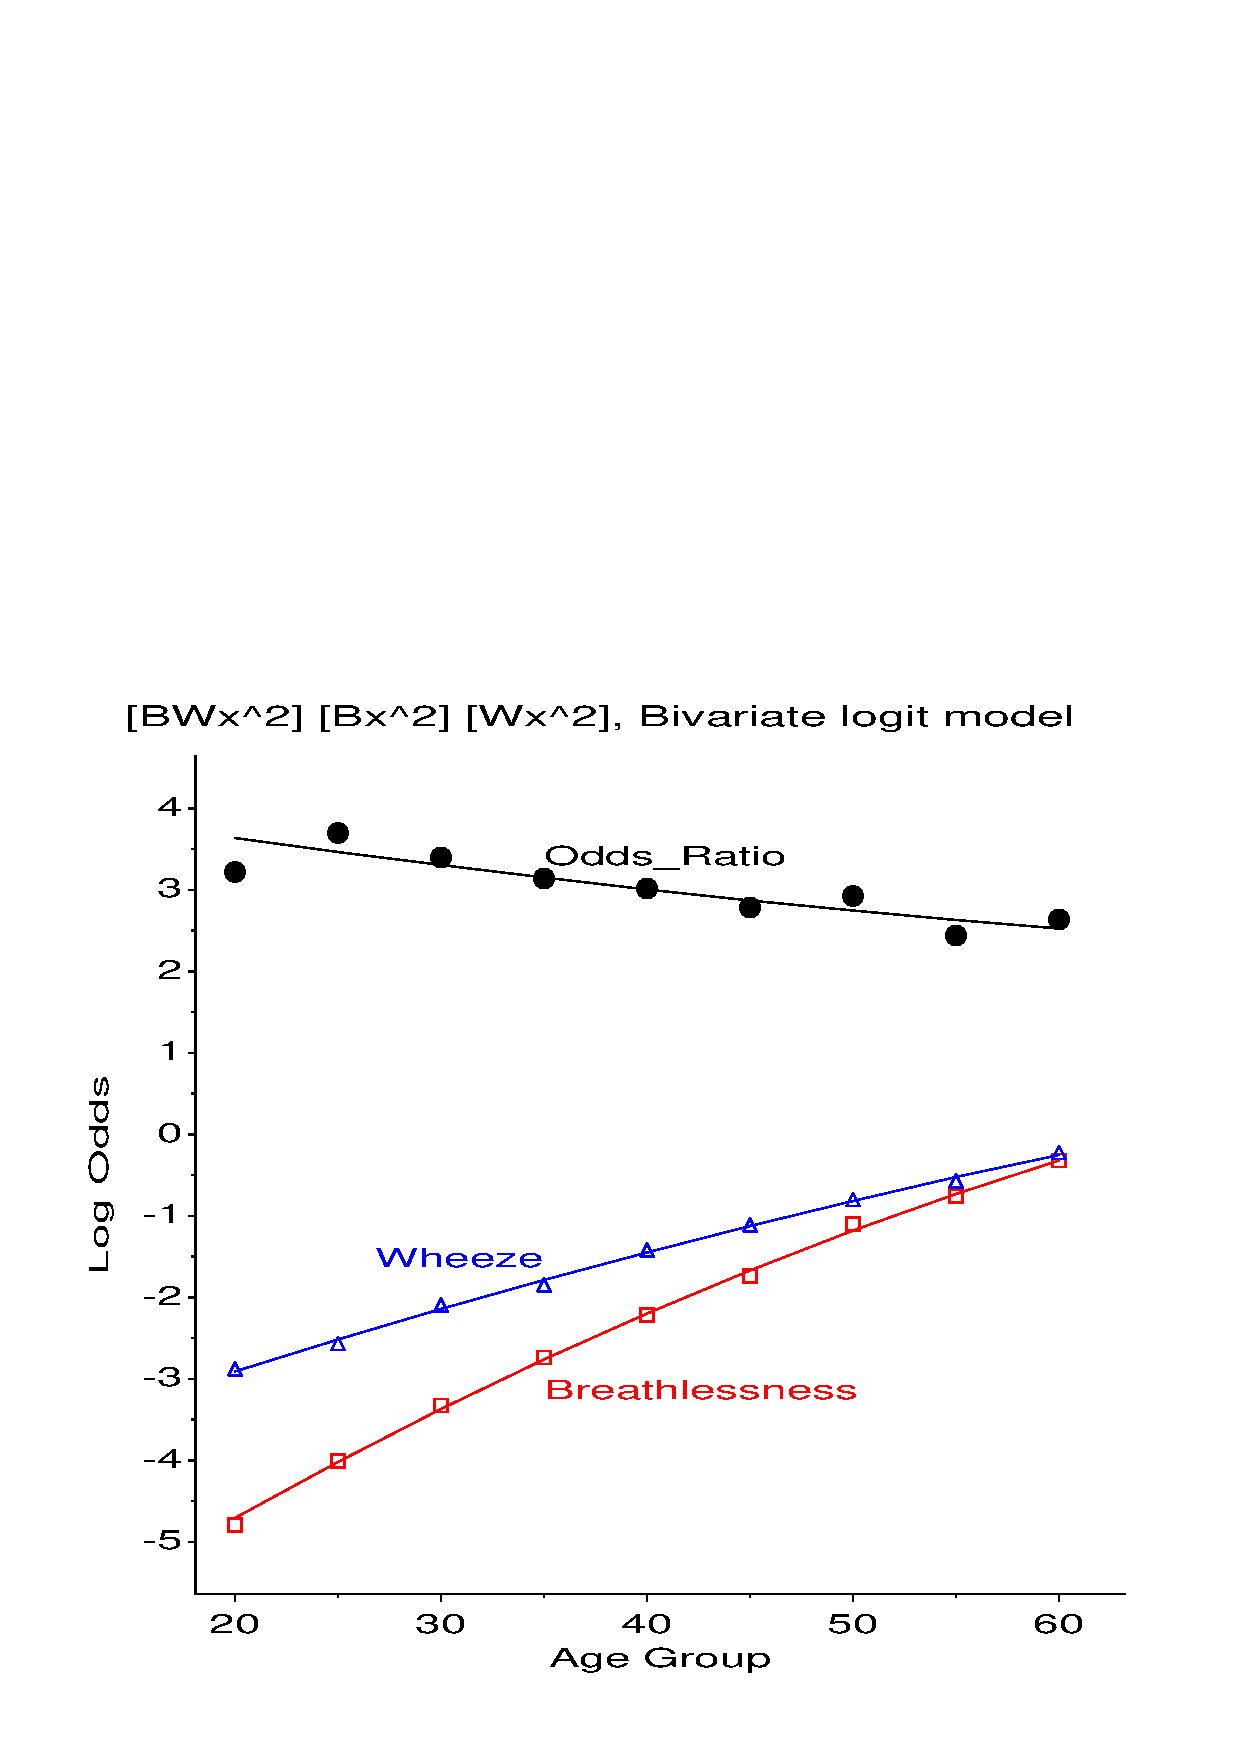
\includegraphics[scale=.6]{ash22}
  \caption[Observed and fitted logits and log odds ratios, quadratic model]{Observed (points) and fitted (curves) logits and log odds ratios for quadratic bivariate logit model}%
  \label{fig:ash22}
\end{figure}

\begin{Output}[htb]
\caption{Model fit and parameter estimates for the linear bivariate logit model }\label{out:ashford.2}
\small
\verbatiminput{ch7/out/ashford.2}
\end{Output}
On statistical grounds, we might be led to choose the quadratic model
as the best fit, but the graphical evidence suggests that the difference
between them is slight.
\figref{fig:ash21} and \figref{fig:ash22} are also both quite similar to the plot
of the empirical logits in \figref{fig:ashford1}, but the fitted models
give a simplified description.
Thus, Model 3 may be summarized as
\begin{equation*}
\left(
\begin{array}{c}
\eta _B \\
\eta _W \\
\eta _{BW}
\end{array}
\right) =\left(
\begin{array}{r}
-6.354 + 0.102 \mbox{ age} \\
-4.089 + 0.065 \mbox{ age} \\
 4.066 - 0.026 \mbox{ age} \\
\end{array}
\right)
\end{equation*}
For each five years, the odds of a miner showing breathlessness are
multiplied by $\exp (5 \times 0.102) = 1.67$, a 67\% increase;
the odds of wheeze increase by  $\exp (5 \times 0.065) = 1.38$, a 38\%
increase.
\end{Example}
